\documentclass[a4paper,12pt]{article}
\usepackage{graphicx} 
\usepackage{amsmath} 

\usepackage{indentfirst}
\usepackage{amsmath} 
\usepackage[varg]{txfonts}
\usepackage{color}
\usepackage{colortbl}
\topmargin=-0.9cm
\oddsidemargin=0.0cm
\evensidemargin=0.0cm
\addtolength{\textheight}{0.5cm}


\definecolor{LemonChiffon}{rgb}{1.,0.98,0.8}
\definecolor{Gold}{rgb}{1.,0.84,0.}
\definecolor{darkblue}{rgb}{0.25,0.,0.95}
\definecolor{lightblue}{rgb}{0.4,0.65,0.95}
\definecolor{grayred}{rgb}{0.7,0.,0.} 
\definecolor{red2}{rgb}{1.0,0.5,0.} 
\definecolor{LemonChiffon}{rgb}{1.,0.98,0.8}
\definecolor{Gold}{rgb}{1.,0.84,0.}
\definecolor{darkblue}{rgb}{0.25,0.,0.95}
\definecolor{lightblue}{rgb}{0.4,0.65,0.95}
\definecolor{RGBblack}{rgb}{0.0,0.0,0.0} 
\def\red{\color{red}}
\def\green{\color{green}}
\def\white{\color{white}}
\def\white{\color{LemonChiffon}}
\def\blue{\color{lightblue}}
\def\gold{\color{Gold}}
\def\black{\color{RGBblack}}



\def\pp{\mathaccent "7F }
\def\p{\mathaccent 95 }


\def\sini {\sin i}
\def\cosi {\cos i}

\def\sino {\sin \Omega}
\def\coso {\cos \Omega}
\def\sinw {\sin \omega}
\def\cosw {\cos \omega}



\begin{document}
\font\norm=cmr12
\font\hugeb=cmb22
\font\isob=cmb18
\font\iso=cmr18
\font\med=cmr14
\font\medb=cmb14
\baselineskip 0.6cm
\parskip\medskipamount
\parskip 0.2cm
\parindent 5mm

%\boldmath

\norm
\hsize 16cm
\vsize 30cm
\newcommand{\bul}{$\bullet \ \ $}
\newcommand{\buu}{\hskip 0.5cm}
\newcommand{\arrow}{$\Rightarrow \ \ $}
\newcommand{\barrow}{\hskip 0.5cm $\Rightarrow \ \ $}
\newcommand{\larrow}{\hskip 0.5cm $\Leftarrow \ \ $}
\newcommand{\hlin}{\vskip 0.5cm}
\newcommand{\hpar}{\vskip 1.0cm}
\newcommand{\nin}{\noindent}
\def\pii{\tilde{\omega}_\circ}

\newcommand{\VV}{$\vec V$ \hskip 0.1cm}
\newcommand{\RR}{$\vec R$ \hskip 0.1cm}

\newcommand{\VVE}{\vec V}
\newcommand{\RRE}{\vec R}

\newcommand{\sverb}{\begin{verbatim}}
\newcommand{\everb}{\end{verbatim}}


%\pagestyle{empty}
{\centerline{}




{\norm
\vskip 0cm
{{\centerline { {\isob CELESTIAL MECHANICS (Fall 2012): }}}}
\vskip 0.2cm
{{\centerline { {\isob COMPUTER EXERCISES II - SOLUTIONS}}}}

{{\centerline { { (Heikki Salo 2.11.2012)}}}}

\vskip 2cm

{\medb 5. Calculation of R and V from orbital elements: 3D case}

{\medb 6. Calculation of orbital elements from R and V}

{\medb 7. Playing with orbits}

\vskip 1cm



These example routines for the solution of the exercises can be copied from


\begin{verbatim}
/wrk/hsalo/TM2012_idl.dir/TM2012_DEMO2.dir
\end{verbatim}

Additional useful procedures:

\begin{verbatim}
/wrk/hsalo/TM2012_idl.dir/TM2012_DEMO1.dir   --  Solutions for exercises I

/wrk/hsalo/TM2012_idl.dir/TM2012_DEMO_apu.dir  --  Useful auxillary programs

\end{verbatim}
\newpage

\black

{\isob 5. Calculation of R and V from orbital elements} \framebox{\bf elem\_to\_rv.pro}


{\red \scriptsize
\begin{verbatim}

;************************************************************
; elem_to_rv.pro
; solves R and V from orbital elements
; HS 6.5.1997 -> 05.11.02 / 01.11.06
;************************************************************
     pro elem_to_rv,elem,time,rad,vel,myy0=myy0,eano=eano,mano=mano

 if(n_params() le 0) then begin
        print,'------------------------------------------------'
        print,'elem_to_rv,elem,time,rad,vel,myy0=myy0'
        print,'     calculates radius- and velocity-vector at a given time 
        print,'     from the orbital elements'
        print,'------------------------------------------------'
        print,' INPUT:'
        print,'  elem = orbital elements [a,eks,ink,ome,w,tau]'
        print,'       a   = semimajor-axis'
        print,'       eks = eccentricity (>1 -> hyperbolic)'
        print,'       ink = inclination'
        print,'       ome = longitude of ascending node'
        print,'       w   = argument of pericenter'
        print,'       tau = time of pericenter passage' 
        print,'       time = instant of time'
        print,'         NOTE: angles in degrees'
        print,' INPUT VIA KEYWORDS:'
        print,'  myy = G (m1+m2)  : def=1'
        print,' OUTPUT:'
        print,'  rad,vel = radius and velocity vector'
        print,' OUTPUT VIA KEYWORDS:'
        print,'   eano=eano eccentric anomaly (degrees)'
        print,'   mano=mano mean anomaly (degrees)'
        print,' HS 6.5.1997 / 22.10.2002 / 01.11.2006 /2008'
        print,'------------------------------------------------'
      return
 endif
       pii=atan(1.d0)*4.d0
       ra=180.d0/pii
       ar=pii/180.d0
       myy=1.d0
       if(keyword_set(myy0)) then myy=myy0
;*************************************************
;     ap=isoakseli                  semimajor axis
;     eps=eksentrisyys              eccentricity
;     ink=inklinaatio               inclination  
;     ome=nousevan solmun pituus    longitude of node
;     w=perihelin argumentti        argument of pericenter
;     tau=periheliaika              pericenter time
;*************************************************
      ap=elem(0)  & eps=elem(1) & ink=elem(2)
      ome=elem(3) & w=elem(4)   & tau=elem(5)  
      ink=ink*ar & ome=ome*ar   & w=w*ar
      bp=ap*sqrt(abs(1.d0-1.d0*eps*eps))

;******************************************************************
;     Orbital vectors ii,jj,kk  
;     (idl-arrays start at zero: here zero-elements are dummies!)
;******************************************************************
     ii=dblarr(4)  & jj=ii & kk=ii     
     sino=sin(ome) & coso=cos(ome)
     sini=sin(ink) & cosi=cos(ink)
     sinw=sin(w)   & cosw=cos(w)
     
     ii(1)=cosw*coso-sinw*sino*cosi
     ii(2)=cosw*sino+sinw*coso*cosi
     ii(3)=sinw*sini
     jj(1)=-sinw*coso-cosw*sino*cosi
     jj(2)=-sinw*sino+cosw*coso*cosi
     jj(3)=cosw*sini
     kk(1)=sino*sini
     kk(2)=-coso*sini
     kk(3)=cosi

;******************************************************************
;mean anomaly
;******************************************************************
     per=2.d0*pii*sqrt(ap*ap*ap/myy)
     m=2.d0*pii/per*(time-tau)

;******************************************************************
;solve eccentric anomaly
;******************************************************************
;cheat a bit: parabolic orbit described by a highly elliptic orbit
 if(eps eq 1) then begin
        eps=.999999
        a=10000.
 endif

;elliptic orbit - Kepler's equation
 if(eps le 1) then begin
        kepler,m,eps,e
     dedt=sqrt(myy/ap^3)/(1.d0-eps*cos(e))
     xx=ap*(cos(e)-eps)
     yy=bp*sin(e)
     vxx=-ap*sin(e)*dedt
     vyy=bp*cos(e)*dedt
     if(e lt 0.) then e=e+!pi*2.d0
 endif

;hyperbolic orbit - hyperbolic Kepler's equation
 if(eps gt 1) then begin
        hkepler,m,eps,e
     dedt=sqrt(myy/ap^3)/(eps*cosh(e)-1.d0)
     xx=ap*(eps-cosh(e))
     yy=bp*sinh(e)
     vxx=-ap*sinh(e)*dedt
     vyy=bp*cosh(e)*dedt
 endif

     mano=m*ra &  eano=e*ra

;******************************************************************
;       convert coordinates from orbit-coordinates
;       to the reference frame
;******************************************************************
     x=xx*ii(1)+yy*jj(1)
     y=xx*ii(2)+yy*jj(2)
     z=xx*ii(3)+yy*jj(3)
     vx=vxx*ii(1)+vyy*jj(1)
     vy=vxx*ii(2)+vyy*jj(2)
     vz=vxx*ii(3)+vyy*jj(3)
     rad=[x,y,z]
     vel=[vx,vy,vz]
    end
\end{verbatim}

\newpage
\black

{\isob 6. Calculation of orbital elements from ${\vec R}$ and ${\vec V}$}
\framebox{\bf rv\_to\_elem.pro}

{\red \scriptsize
\begin{verbatim}

;*********************************************************
; rv_to_elem.pro
; solves orbital elements from radius and velocity vectors
; HS 6.5.1997 -> 05.11.02 -> 01.11.06
;*********************************************************

pro rv_to_elem,time,rad,vel,elem,$
               print=print,myy0=myy0,kvec=kvec,evec=evec,$
               ene=ene,imp=imp,eano=eano,mano=mano

if(n_params() le 0) then begin
 print,'------------------------------------------------'
 print,'pro rv_to_elem,time,rad,vel,elem'
 print,'    calculates orbital elements from radius and velocity vectors'
 print,'    at a given time'
 print,'------------------------------------------------'
 print,' INPUT:'
 print,'  time = time of observation'
 print,'  rad = [ x, y, z] radius vector'
 print,'  vel = [vx,vy,vz] velocity vector'
 print,' INPUT VIA KEYWORDS:'
 print,'  myy = value   - def: G*(m1+m2) = 1.'
 print,' '
 print,' OUTPUT:'
 print,'  elem=[a,eks,ink,ome,w,tau]'
 print,'       a   = semimajor-axis'
 print,'       eks = eccentricity (>1 -> hyperbolic)'
 print,'       ink = inclination'
 print,'       ome = longitude of ascending node'
 print,'       w   = argument of pericenter'
 print,'       tau = time of pericenter passage' 
 print,' OUTPUT VIA KEYWORDS:'
 print,'  kvec=kvector =[kx,ky,kz]'
 print,'  evec=evector =[ex,ey,ez]'
 print,'  imp=angular momentum/unit mass = |kvec|'
 print,'  ene=energy /unit mass'
 print,'  eano=eccentric anomaly (degrees)'
 print,'  mano=mean anomaly (degrees)'
 print,' '
 print,' ADDITIONAL KEYWORDS:'
 print,'  /print -> some intermediate output'
 print,' HS 6.5.1997 / 22.10.2002 /01.11.2006'
 print,'  '
 return
endif

;defines units
 myy=1.d0
 if(keyword_set(myy0)) then myy=myy0

 pii=atan(1.d0)*4.d0
 ra=180.d0/pii
 ar=pii/180.d0
 
;*************************************************
; inklinaatio ja nousevan solmun pituus
; inclination and the longitude of ascending node
;*************************************************
; cross_product,A,B,C    --> C = A x B    
; dot_product,A,B,c      --> c = A . B   
; here A,B,C denote 3-element vectors, c denotes a scalar
; angle=atan(y,x) returns angle for which y=sin(angle), x=cos(angle)

 cross_product,rad,vel,kvec
 dot_product,kvec,kvec,kk
 n=kvec/sqrt(kk)
 nx=n(0)
 ny=n(1)
 nz=n(2)
 ink=acos(nz)
 ome=atan(nx,-ny)
 imp=sqrt(kk)

;*************************************************
; eksentrisyys ja perihelin argumentti: e-VEKTORI
; eccentricity and the argument of pericenter
;*************************************************

 cross_product,kvec,vel,apu1
 dot_product,rad,rad,r2
 apu2=rad/sqrt(r2)
 evec=-apu1/myy-apu2

;transform evec to the coordinate system aligned
;with the orbital plane

 coso=cos(ome)
 sino=sin(ome)
 cosi=cos(ink)
 sini=sin(ink)

 ex=coso*evec(0)+sino*evec(1)
 ey=-sino*cosi*evec(0)+coso*cosi*evec(1)+sini*evec(2)

 eks=sqrt(ex^2+ey^2)
 w=atan(ey,ex)

;************************************************
;isoakseli 
;semimajor axis
;************************************************

 dot_product,vel,vel,v2
 dist=sqrt(r2)
 h=0.5d0*v2-myy/sqrt(r2)
 ene=h
 a=abs(myy/2.d0/h)
 per=2.0d0*!dpi*sqrt(a^3/myy)

;************************************************
; periheliaika
; time of pericenter passage
;************************************************
;via cos(E) 
;to solve the right sign:

;0   <E < 180 -> r is increasing
;180 <E < 360 -> r is decreasing

 sign=1.
 dot_product,rad,vel,rv
 if(rv lt 0.) then sign=-1.

;******************************************
;elliptic orbit
;just to avoid numerical problems:
 if(eks le 0.) then begin
   e=0.
   m=e
   tau=time
 endif
 if(eks lt 1. and eks gt 0.) then begin
   cose=(1.-dist/a)/eks<1.d0>(-1.d0)
   e=acos(cose)*sign
   m=e-eks*sin(e)
   tau=(time-m*per/2./!dpi) mod per
 endif

;******************************************
;hyperbolic orbit
;acosh-function returns the inverse of hyperbolic cosine
;(in acosh.pro)

 if(eks ge 1.) then begin
   coshe=(1.d0+dist/a)/eks>1.
   e=acosh(coshe)*sign
   m=eks*sinh(e)-e
   tau=time-m*per/2./!pi
 endif

 eano=e*!radeg
 mano=m*!radeg
 elem=[a,eks,ink*!radeg,ome*!radeg,w*!radeg,tau]

 if(keyword_set(print)) then begin
   st=' at T='+string(time)
   print,'-------------------------------------------------'
   if(eks lt 1) then print,'CALCULATED ELEMENTS OF ELLIPTIC ORBIT:'+st
   if(eks gt 1) then print,'CALCULATED ELEMENTS OF HYPERBOLIC ORBIT:'+st
   print,'a   = ',elem(0)
   print,'eks = ',elem(1)
   print,'ink = ',elem(2)
   print,'ome = ',elem(3)
   print,'w   = ',elem(4)
   print,'tau = ',elem(5)
   print,' '
   print,'per = ',per,m*ra
   print,'q   = ',elem(0)*abs(1.-elem(1))
   print,' '
   print,'-------------------------------------------------'
endif

end

\end{verbatim}
\black}


\newpage
\black

{\medb
Procedure for solving Kepler's equation for hyperbolic orbits} \framebox{\bf hkepler.pro}


{\red \scriptsize
\begin{verbatim}

;***************************************************************
;     RATKAISTAAN HYBERPOLINEN EKSENTRINEN ANOMALIA E
;     ITEROIMALLA KESKIANOMALIASTA M
;     RADAN EKSENTRISYYS = EKS > 1
;***************************************************************

     pro hkepler,m,eks,e,itul=itul,itemax=itemax,check=check

;***************************************************************
   if(n_params() le 0) then begin
       print,'---------------------------------------------'
       print,' hkepler,M,eks,E'
       print,'---------------------------------------------'
       print,' SOLVES KEPLER-EQUATION for HYPERBOLIC ORBIT
       print,' M = eks*sinh(E) - E,    eks>1' 
       print,' USING NEWTON-ITERATION'
       print,' input:   M = mean anomaly (radians), eks=eccentricity '
       print,' output:  E = eccentric anomaly (radians)'
       print,' keywords: '
       print,'   /itul  -> output iteration values (E)'
       print,'   /check -> check accuracy of solution'
       print,'   itemax =  max number of iterations (def=500)'
       print,' example:  eks=3, M= 45 degrees, output iteration values'
       print,"   hkepler,45./!radeg,3.,e,/itul & print,'E=',e*!radeg,' deg'"
       print,' HS 04.10.02 /01.11.06'
       print,'---------------------------------------------'
   return
 endif
;***************************************************************
;Newton iteration for solving  f=eks*sinh(E)- E - M = 0
; E_NEW = E_OLD - f(E)/(df(E)/dE)
; until abs(E_NEW-E_OLD) < 1d-10

     nstep=5000
     if(keyword_set(itemax)) then nstep=itemax

;choose the intitial guess
     e=m
     if(abs(m) gt exp(1)) then e=m/abs(m)*alog(2.*abs(m)/eks)

     i=0
     if(keyword_set(itul)) then print,i,e
     for i=1,nstep do begin
            fe=eks*sinh(e)-e-m
            fep=eks*cosh(e)-1.d0
            eold=e
            e=eold-fe/fep
            if(abs(e-eold) lt 1d-10*abs(e)) then goto,jump11
            if(keyword_set(itul)) then print,i,e
        endfor
        jump11: 
        if(keyword_set(check)) then print,m-(eks*sinh(e)-e)
     return
     end


\end{verbatim}
\black}

\newpage
\black
{\medb
Auxillary routines
}
\vskip 0.5cm

\bul ACOSH \framebox{\bf acosh.pro}
{\red \scriptsize
\begin{verbatim}
;acosh.pro
;hyperbolisen cosinin kaanteisfunktio 
;y=cosh(x)=0.5*(exp(x)+exp(-x)) --> x=acosh(y)
;HS circa 1997
function acosh,y
  x=alog(y+sqrt(y^2-1))
return,x
end


\end{verbatim}
\black}

\bul VECTOR PRODUCT \framebox{\bf cross\_product.pro}
{\red \scriptsize
\begin{verbatim}
;***************************
;cross_product.pro 
;***************************
pro cross_product,a,b,c

if(n_params(0) le 0) then begin
    print,'----------------------------------------------'
    print,' pro cross_product,A,B,C'
    print,' C=A x B'
    print,'----------------------------------------------'
    print,' case 1: A and B are 3-element vectors:'
    print,'   A=[ax,ay,az], B=[bx,by,bz]] -> C=[cx,cy,cz]'
    print,'----------------------------------------------'
    print,' case 2: A and B contain an array of 3-element vectors'
    print,'   A=array(n,3) B=array(n,3) -> C=array(n,3)'
    print,'----------------------------------------------'
    print,'HS ca 2000'
    return
endif

;case 1
if(n_elements(a) eq 3) then begin
    c=a
    c(0)=a(1)*b(2)-b(1)*a(2)
    c(1)=a(2)*b(0)-b(2)*a(0)
    c(2)=a(0)*b(1)-b(0)*a(1)
endif

;case 2
if(n_elements(a) gt 3) then begin
    n=n_elements(a)/3
    c=a
    c(*,0)=a(*,1)*b(*,2)-b(*,1)*a(*,2)
    c(*,1)=a(*,2)*b(*,0)-b(*,2)*a(*,0)
    c(*,2)=a(*,0)*b(*,1)-b(*,0)*a(*,1)
endif

return
end
\end{verbatim}
\black}

\newpage

\bul SCALAR PRODUCT \framebox{\bf dot\_product.pro}
{\red \scriptsize
\begin{verbatim}
;***************************
;dot_product.pro
;scalar-product c = a . b
;***************************

pro dot_product,a,b,c

if(n_params(0) le 0) then begin
    print,'----------------------------------------------'
    print,' pro dot_product,A,B,c'
    print,' scalar product c = A . B'
    print,'----------------------------------------------'
    print,' case 1: A and B are 3-element vectors:'
    print,'   A=[ax,ay,az], B=[bx,by,bz]] -> c =ax*bx+ay*by+az*bz'
    print,'----------------------------------------------'
    print,' case 2: A and B contain an array of 3-element vectors'
    print,'   A=array(n,3) B=array(n,3) -> c=array(n)'
    print,'----------------------------------------------'
    print,'HS ca 2000'
    return
endif

;case 1
if(n_elements(a) eq 3) then begin
    c=a(0)*b(0)+a(1)*b(1)+a(2)*b(2)
endif

;case 2
if(n_elements(a) gt 3) then begin
    n=n_elements(a)/3
    c=a(*,0)
    c=a(*,0)*b(*,0)+a(*,1)*b(*,1)+a(*,2)*b(*,2)
endif

return
end

\end{verbatim}
\black}

\newpage

{\isob Checking elem\_to\_rv.pro  and  rv\_to\_elem.pro }\framebox{\bf elem\_rv\_example.pro}


{\red \scriptsize
\begin{verbatim}

;**********************************************************
;elem_rv_example.pro
;**********************************************************
;example of using the procedures
;   elem_to_rv  : orbital elements -> R,V  at given t
;   rv_to_elem  : R,V at given t -> orbital elements
;HS 22.10.2002/01.11.06
;**********************************************************

   print,'--------------------------------------------------'
   print,'CHECK THE PROCEDURES:'
   print,' elem_to_rv  : orbital elements -> R,V  at given t'
   print,' rv_to_elem  : R,V at given t -> orbital elements '
   print,'--------------------------------------------------'

;******************************************************
;ELLIPTIC ORBIT
;******************************************************
   a=1.7                        ;semimajor axis
   eks=0.1                      ;eccentricity
   ink=10.                      ;inclination
   ome=40.                      ;longitude of ascending node
   w=20.                        ;argument of pericenter
   tau=0.1                      ;time of pericenter passage 
   elem0=[a,eks,ink,ome,w,tau]

   time=0.7
   elem_to_rv,elem0,time,rad,vel
   rv_to_elem,time,rad,vel,elem1

   print,'original elements: elliptic orbit'
   print,'         a         eks        ink         ome          w         tau'
   print,elem0,f='(6f12.6)'
   print,'new elements'
   print,elem1,f='(6f12.6)'
      
;******************************************************
;HYPERBOLIC ORBIT
;******************************************************

   a=1.7                        ;semimajor axis
   eks=1.1                      ;eccentricity
   ink=10.                      ;inclination
   ome=40.                      ;longitude of ascending node
   w=20.                        ;argument of pericenter
   tau=0.1                      ;time of pericenter passage 
   elem0=[a,eks,ink,ome,w,tau]

   time=0.7
   elem_to_rv,elem0,time,rad,vel
   rv_to_elem,time,rad,vel,elem1

   print,'--------------------------------------------------'
   print,'original elements: hyperbolic orbit'
   print,'         a         eks        ink         ome          w         tau'
   print,elem0,f='(6f12.6)'
   print,'new elements'
   print,elem1,f='(6f12.6)'
   print,'--------------------------------------------------'
end
\end{verbatim}
\black}


This code should produce output:

{\red \scriptsize
\begin{verbatim}

--------------------------------------------------
CHECK THE PROCEDURES:
 elem_to_rv  : orbital elements -> R,V  at given t
 rv_to_elem  : R,V at given t -> orbital elements
--------------------------------------------------
original elements: elliptic orbit
         a         eks        ink         ome          w         tau
    1.700000    0.100000   10.000000   40.000000   20.000000    0.100000
new elements
    1.700000    0.100000    9.999999   39.999998   19.999992    0.100000
--------------------------------------------------
original elements: hyperbolic orbit
         a         eks        ink         ome          w         tau
    1.700000    1.100000   10.000000   40.000000   20.000000    0.100000
new elements
    1.700000    1.100000    9.999999   39.999998   19.999997    0.100000
--------------------------------------------------


\end{verbatim}
\black}



\newpage

\black
{\isob 7. Playing with orbits}

{\medb a) Procedure for calculating/plotting an orbit} ~~ \framebox{\bf elem\_orbit.pro}


{\red \scriptsize
\begin{verbatim}
;*****************************************************
; elem_orbit.pro
; use elem_to_rv to calculate orbit
; HS 05.11.02 /01.11.2006
;*****************************************************

pro elem_orbit,elem,timet,rr,vv,myy0=myy0,plot=plot

  if(n_params() le 0) then begin
      print,'elem_orbit,elem,timet,rr,vv,myy0=myy0'
      print,'elem = orbital elements [a,eks,ink,ome,w,tau]'
      print,'timet -> calculate RR(*,3)  VV(*,3) for these times'
      print,'myy   -> scaling (def=1.)'
      print,'plot=1 ->  plot x,y orbit'
      print,'plot>1 -> oplot x,y orbit with col=plot'
      print,'----------------------------'
      print,'Example:'
      print,'timet=findgen(101)/100.*2*!pi & !x.range=[-2,2] & !y.range=[-2,2]'
      print,'elem_orbit,[1.,.0,0.,0.,0.,0.],timet,/plot'
      print,'elem_orbit,[1.,.5,0.,0.,0.,0.],timet, plot=2'
      print,'elem_orbit,[1.,.9,0.,0.,0.,0.],timet, plot=3'
      return
  endif
;*****************************************************
;choose scaling
  myy=1
  if(keyword_set(myy0)) then myy=myy0
 ;*****************************************************
;orbital position vector R and velocity vector R are calculated
;for times defined in call
;rr and vv contain position and velocity components
    ntimet=n_elements(timet)
    rr=findgen(ntimet,3)
    vv=findgen(ntimet,3)

  for i=0,ntimet-1 do begin
    time=timet(i)
    elem_to_rv,elem,time,rad,vel,myy=myy
    rr(i,0)=rad(0)
    rr(i,1)=rad(1)
    rr(i,2)=rad(2)
    vv(i,0)=vel(0)
    vv(i,1)=vel(1)
    vv(i,2)=vel(2)
  endfor

if(keyword_set(plot)) then begin
    if(plot eq 1) then begin  
        nwin
        plot,rr(*,0),rr(*,1),xtitle='x',ytitle='y',/iso,psym=3
        plots,0,0,psym=1
    endif
    if(plot gt 1) then begin          
        oplot,rr(*,0),rr(*,1),col=plot,psym=3
    endif
endif
end

\end{verbatim}
\black}

\newpage

\black Example output form \framebox{\bf elem\_orbit.pro}


Enter in IDL workspace the following lines:
\red
\begin{verbatim}
 timet=findgen(101)/100.*2*!pi & !x.range=[-2,2]  & !y.range=[-2,2]
 elem_orbit,[1.,.0,0.,0.,0.,0.],timet,/plot
 elem_orbit,[1.,.5,0.,0.,0.,0.],timet, plot=2
 elem_orbit,[1.,.9,0.,0.,0.,0.],timet, plot=3
\end{verbatim}
\black

This should make a plot:

\vspace{-14cm}
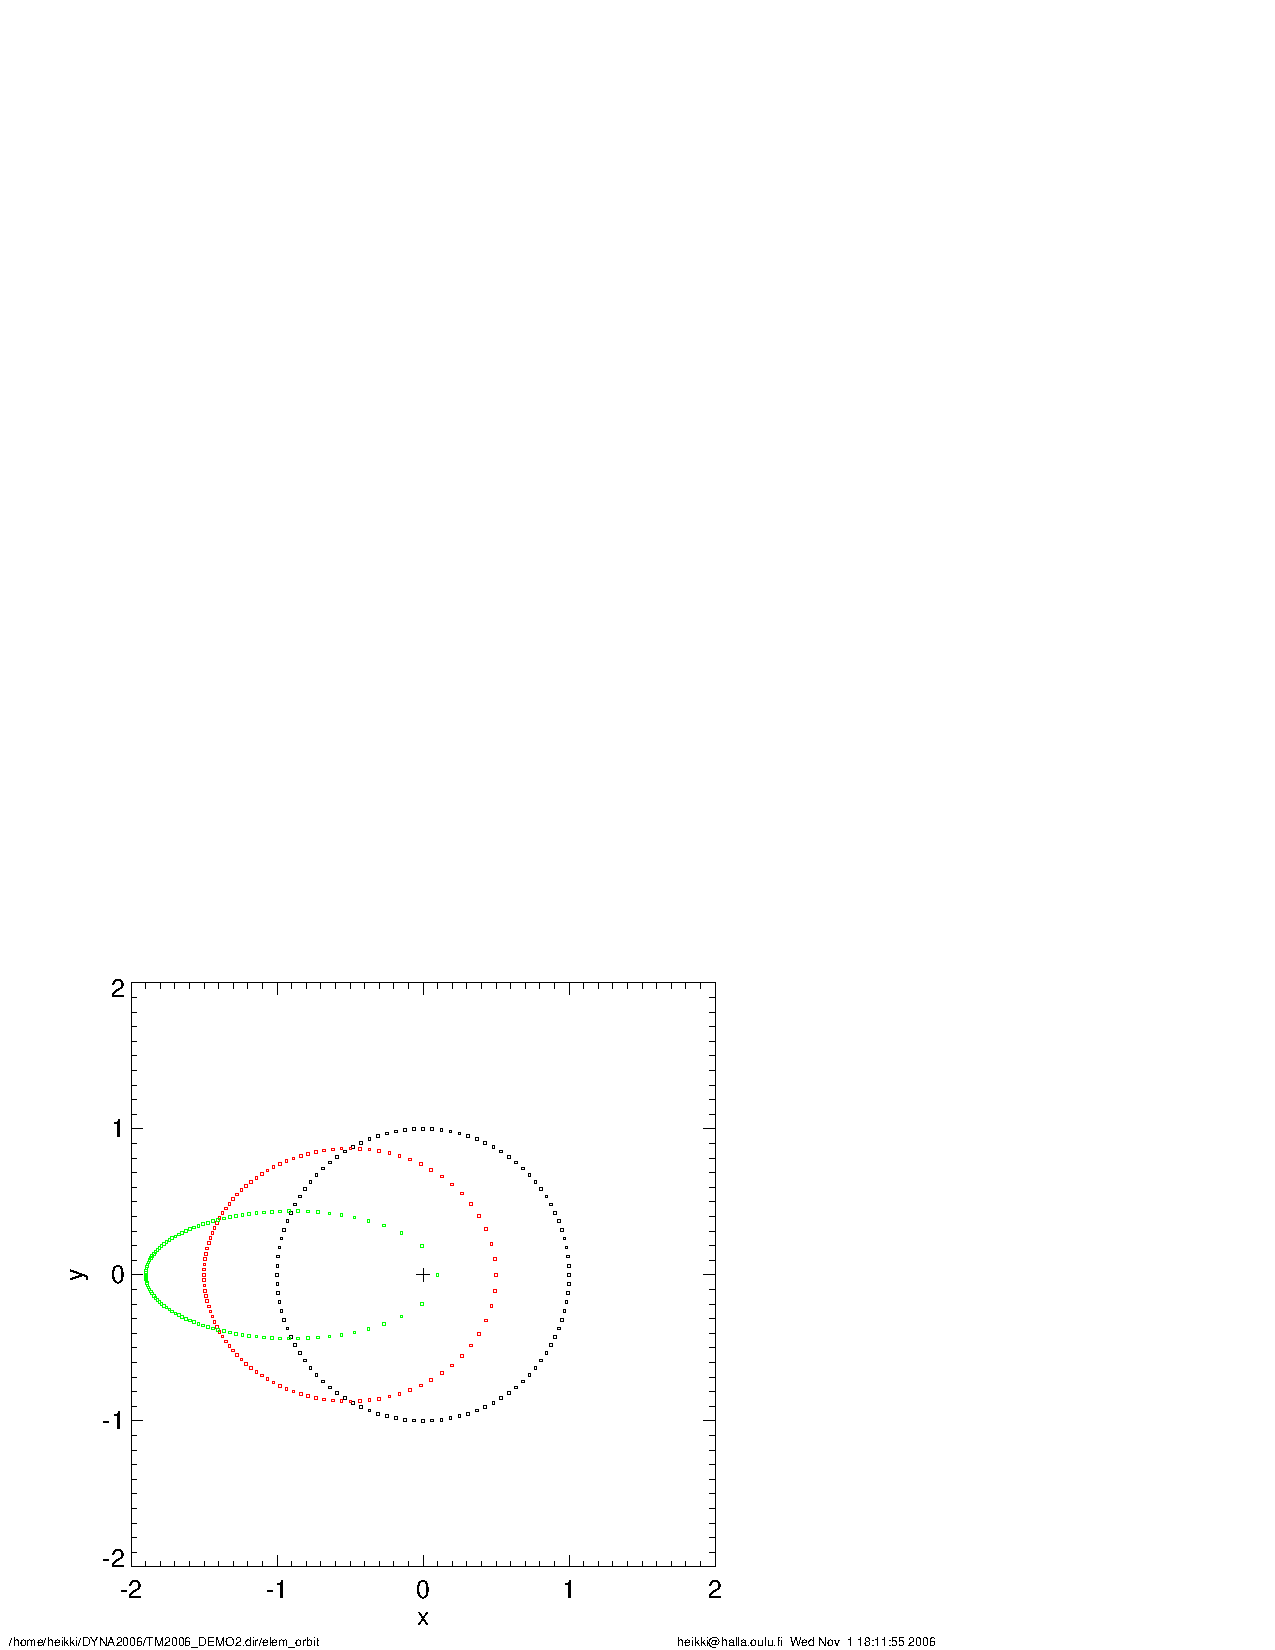
\includegraphics[width=1\paperwidth]{elem_orbit.pdf}






\newpage
\black
{\medb b) Satellite launched from Earth} 


\bul \framebox{\tt elem\_orbit\_demo\_tangential.pro}  -- tangential velocity increments (max=30km/sec)

\bul \framebox{\tt elem\_orbit\_demo\_radial.pro}  -- radial velocity increments 

\bul \framebox{\tt elem\_orbit\_demo\_vertical.pro}  -- vertical velocity increments


Just the first one is printed here, since the other two are almost similar


{\red \scriptsize
\begin{verbatim}
;*****************************************************
; elem_orbit_demo_tangential.pro
; use elem_orbit to plot orbits with different elements
; elem = orbital elements [a,eks,ink,ome,w,tau]
; HS 05.11.02 /01.11.06
;**************************************************************
;   Earth position (AU) and velocity (km/sec)
;   assuming circular orbit with velocity 30 km/sec

       r_earth=[1.,0.,0.]
       v_earth= [0.,30.,0.]

;   units: AU and year -> G(m1+m2)=4*pi^2
;   orbital speed of Earth = 30 km/sec   = 2*pi AU/year
;   km/sec converted to au/year by multiplying with vscale=(2*pi)/30.

      myy=4.*!pi^2         ;yksikot AU, vuosi
      vscale=(2.*!pi)/30.  ;muuntaa km/sec -->  AU/vuosi

;give here different tangential velocity increments (norb different ones)
      norb=16
      dv=findgen(norb)*2
      norb=n_elements(dv)
      vx=v_earth(0)+dv*0.
      vy=v_earth(1)+dv
      vz=v_earth(2)+dv*0.
      title='tangential velocity increments, max='+string(max(dv))+'km/sec'
;*************************************************************
;1) calculate and store orbital elements
;   rv_to_elem returns: elem=[a,eks,ink,ome,w,tau]
;   also store the orbital energy (ene)
;*************************************************************
      elem_tab=fltarr(6,norb)   ; norb different orbits
      ene_tab=fltarr(norb)
      ene_earth=abs(myy/2.)     ; Maan energia 

 print,'Satellite launched from Earth orbit (v_cir=30km/sec)'
 print,'----------------------------------------------------------------------'
 print,'dv_tan     a     eks      ink     ome       w     tau  ene/|ene_earth|'
 print,'----------------------------------------------------------------------'
 ff='(f4.1,2x, 2f8.3, 4f8.1, 2x,f9.3)'

    for i=0,norb-1 do begin
        v=[vx(i),vy(i),vz(i)]
        r=r_earth
        v=v*vscale
;orbital elements
        rv_to_elem,0.,r,v,elem,myy=myy,ene=ene
        print,dv(i),elem,ene/ene_earth,f=ff
        elem_tab(*,i)=elem
        ene_tab(i)=ene
     endfor
 print,'----------------------------------------------------------------------'

;*****************************************
;2) calculate and plot orbits
;*****************************************
   nwin
   timet=findgen(1000)/100.   ; 0-9 years
   for i=0,norb-1 do begin
       elem=elem_tab(*,i)
       elem_orbit,elem,timet,rr,vv,myy=myy
       if(i eq 0) then begin
          plot,rr(*,0),rr(*,1),psym=3,xtitle='x',ytitle='y',$
               xr=[-5,5]-3,yr=[-5,5],xs=1,ys=1,/iso,title=title
          plots,0,0,psym=1
       endif
       if(i ne 0) then oplot,rr(*,0),rr(*,1),psym=3,col=i+1
    endfor
    xyouts,0.01,0.01,/normal,'elem_orbit_demo.pro',chars=.75

;*****************************************
;3) plot energy/|energy vs |dv|/|v_earth|
;*****************************************
     nwin
     plot,dv/30.,ene_tab/ene_earth,xtit='|dv|/|v_earth|',ytit='ene/|ene_Earth|'
;indicate the limit for hyperbolic orbit
     oplot,[0,1],[0,0],lines=1
     oplot,(sqrt(2)-1)*[1,1],[-1,2],lines=1
     xyouts,0.01,1.8,'|dv|/v_circ=sqrt(2)-1 --> v/v_circ=sqrt(2)'
     xyouts,0.01,0.01,/normal,'elem_orbit_demo.pro',chars=.75
end

\end{verbatim}
\black}
\small

\newpage

{\medb output:  tangential, radial, vertical velocity increments:}

\vspace{-9cm}
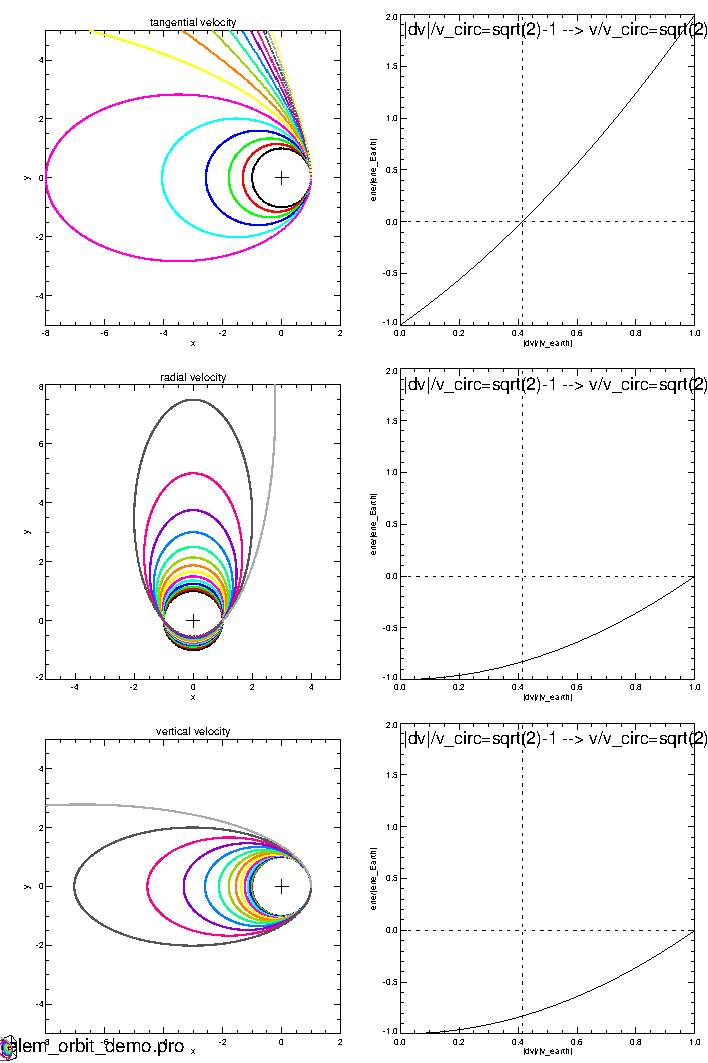
\includegraphics[height=1.4\paperwidth]{demo_apu.pdf}


\newpage





{\red \scriptsize
\begin{verbatim}  
TANGENTIAL VELOCITY INCREMENT
----------------------------------------------------------------------
dv_tan     a     eks      ink     ome       w     tau  ene/|ene_earth|
----------------------------------------------------------------------
 0.0     1.000   0.000     0.0   180.0     0.0     0.0     -1.000
 2.0     1.160   0.138     0.0   180.0   180.0     0.0     -0.862
 4.0     1.398   0.284     0.0   180.0   180.0    -0.0     -0.716
 6.0     1.786   0.440     0.0   180.0   180.0     0.0     -0.560
 8.0     2.528   0.604     0.0   180.0   180.0     0.0     -0.396
10.0     4.500   0.778     0.0   180.0   180.0     0.0     -0.222
12.0    25.000   0.960     0.0   180.0   180.0     0.0     -0.040
14.0     6.618   1.151     0.0   180.0   180.0    -0.0      0.151
16.0     2.848   1.351     0.0   180.0   180.0     0.0      0.351
18.0     1.786   1.560     0.0   180.0   180.0    -0.0      0.560
20.0     1.286   1.778     0.0   180.0   180.0    -0.0      0.778
22.0     0.996   2.004     0.0   180.0   180.0    -0.0      1.004
24.0     0.806   2.240     0.0   180.0   180.0     0.0      1.240
26.0     0.674   2.484     0.0   180.0   180.0    -0.0      1.484
28.0     0.575   2.738     0.0   180.0   180.0    -0.0      1.738
30.0     0.500   3.000     0.0   180.0   180.0     0.0      2.000
----------------------------------------------------------------------
RADIAL  VELOCITY INCREMENTS
----------------------------------------------------------------------
dv_rad     a     eks      ink     ome       w     tau  ene/|ene_earth|
----------------------------------------------------------------------
 0.0     1.000   0.000    0.00  180.00    0.00    0.00     -1.000
 2.0     1.004   0.067    0.00  180.00   90.00   -0.23     -0.996
 4.0     1.018   0.133    0.00  180.00   90.00   -0.21     -0.982
 6.0     1.042   0.200    0.00  180.00   90.00   -0.20     -0.960
 8.0     1.077   0.267    0.00  180.00   90.00   -0.19     -0.929
10.0     1.125   0.333    0.00  180.00   90.00   -0.17     -0.889
12.0     1.190   0.400    0.00  180.00   90.00   -0.16     -0.840
14.0     1.278   0.467    0.00  180.00   90.00   -0.15     -0.782
16.0     1.398   0.533    0.00  180.00   90.00   -0.15     -0.716
18.0     1.562   0.600    0.00  180.00   90.00   -0.14     -0.640
20.0     1.800   0.667    0.00  180.00   90.00   -0.13     -0.556
22.0     2.163   0.733    0.00  180.00   90.00   -0.13     -0.462
24.0     2.778   0.800    0.00  180.00   90.00   -0.12     -0.360
26.0     4.018   0.867    0.00  180.00   90.00   -0.12     -0.249
28.0     7.759   0.933    0.00  180.00   90.00   -0.11     -0.129
30.0  Infinity   1.000    0.00  180.00   90.00    -NaN      0.000
----------------------------------------------------------------------
VERTICAL VELOCITY INCREMENT
----------------------------------------------------------------------
dv_ver     a     eks      ink     ome       w     tau  ene/|ene_earth|
----------------------------------------------------------------------
 0.0     1.000   0.000    0.00  180.00    0.00    0.00     -1.000
 2.0     1.004   0.004    3.81    0.00   -0.00   -0.00     -0.996
 4.0     1.018   0.018    7.59    0.00   -0.00   -0.00     -0.982
 6.0     1.042   0.040   11.31    0.00   -0.00    0.00     -0.960
 8.0     1.077   0.071   14.93    0.00   -0.00    0.00     -0.929
10.0     1.125   0.111   18.43    0.00   -0.00    0.00     -0.889
12.0     1.190   0.160   21.80    0.00   -0.00    0.00     -0.840
14.0     1.278   0.218   25.02    0.00   -0.00    0.00     -0.782
16.0     1.398   0.284   28.07    0.00   -0.00   -0.00     -0.716
18.0     1.562   0.360   30.96    0.00   -0.00   -0.00     -0.640
20.0     1.800   0.444   33.69    0.00   -0.00   -0.00     -0.556
22.0     2.163   0.538   36.25    0.00   -0.00    0.00     -0.462
24.0     2.778   0.640   38.66    0.00   -0.00    0.00     -0.360
26.0     4.018   0.751   40.91    0.00   -0.00    0.00     -0.249
28.0     7.759   0.871   43.03    0.00   -0.00   -0.00     -0.129
30.0  Infinity   1.000   45.00    0.00   -0.00    -NaN      0.000
----------------------------------------------------------------------
\end{verbatim}
\black}

\newpage
\black

An attempt to visualize 3D-orbits: (extract from {\tt elem\_orbit\_demo\_vertical.pro})
{\red \scriptsize 
\begin{verbatim}
;***************************************************
;4) calculate and plot orbits, using 3d-plot
;***************************************************
;use shade-surface to make the viewing transformation 
;and draw a box with the size lim
  
  lim=2
  x=findgen(6)/5.*20
  surface,x#x,x,x,/save,xr=[-1,1]*lim,yr=[-1,1]*lim,zr=[-1,1]*lim,/nod,$
  xs=1,ys=1,zs=1,pos=[.15,.1,.85,.9],xtit='X',ytit='Y',ztit='Z',chars=1.5,$
  title=title

  x=lim*[-1,1,1,-1,-1,1,1,-1] &  y=lim*[-1,-1,1,1,-1,-1,1,1] & z=lim*[-1,-1,-1,-1,1,1,1,1]
  front=[0,1,2,3,0] &  back=[4,5,6,7,4]
  ls=2
  plots,x(front),y(front),z(front),/t3d,/data,linestyle=ls
  plots,x(back),y(back),z(back),/t3d,/data,linestyle=2
  for i=0,3 do begin
    side=[i,i+4]
    plots,x(side),y(side),z(side),/t3d,/data,linestyle=2
  endfor

;calculate and plot orbits
 timet=findgen(1000)/100.   ; 0-9 years
 for i=0,npart-1 do begin
   elem=elem_tab(*,i)
   elem_orbit,elem,timet,rr,vv,myy=myy
   plots,rr(*,0),rr(*,1),rr(*,2),psym=3,/t3d,col=i+1
   index=where(rr(*,2) gt 0, count)
   if(count gt 0) then plots,rr(index,0),rr(index,1),rr(index,2),psym=6,$
                  /t3d,col=i+1,syms=.5
 endfor
\end{verbatim}
\black}



\vspace{-8cm}
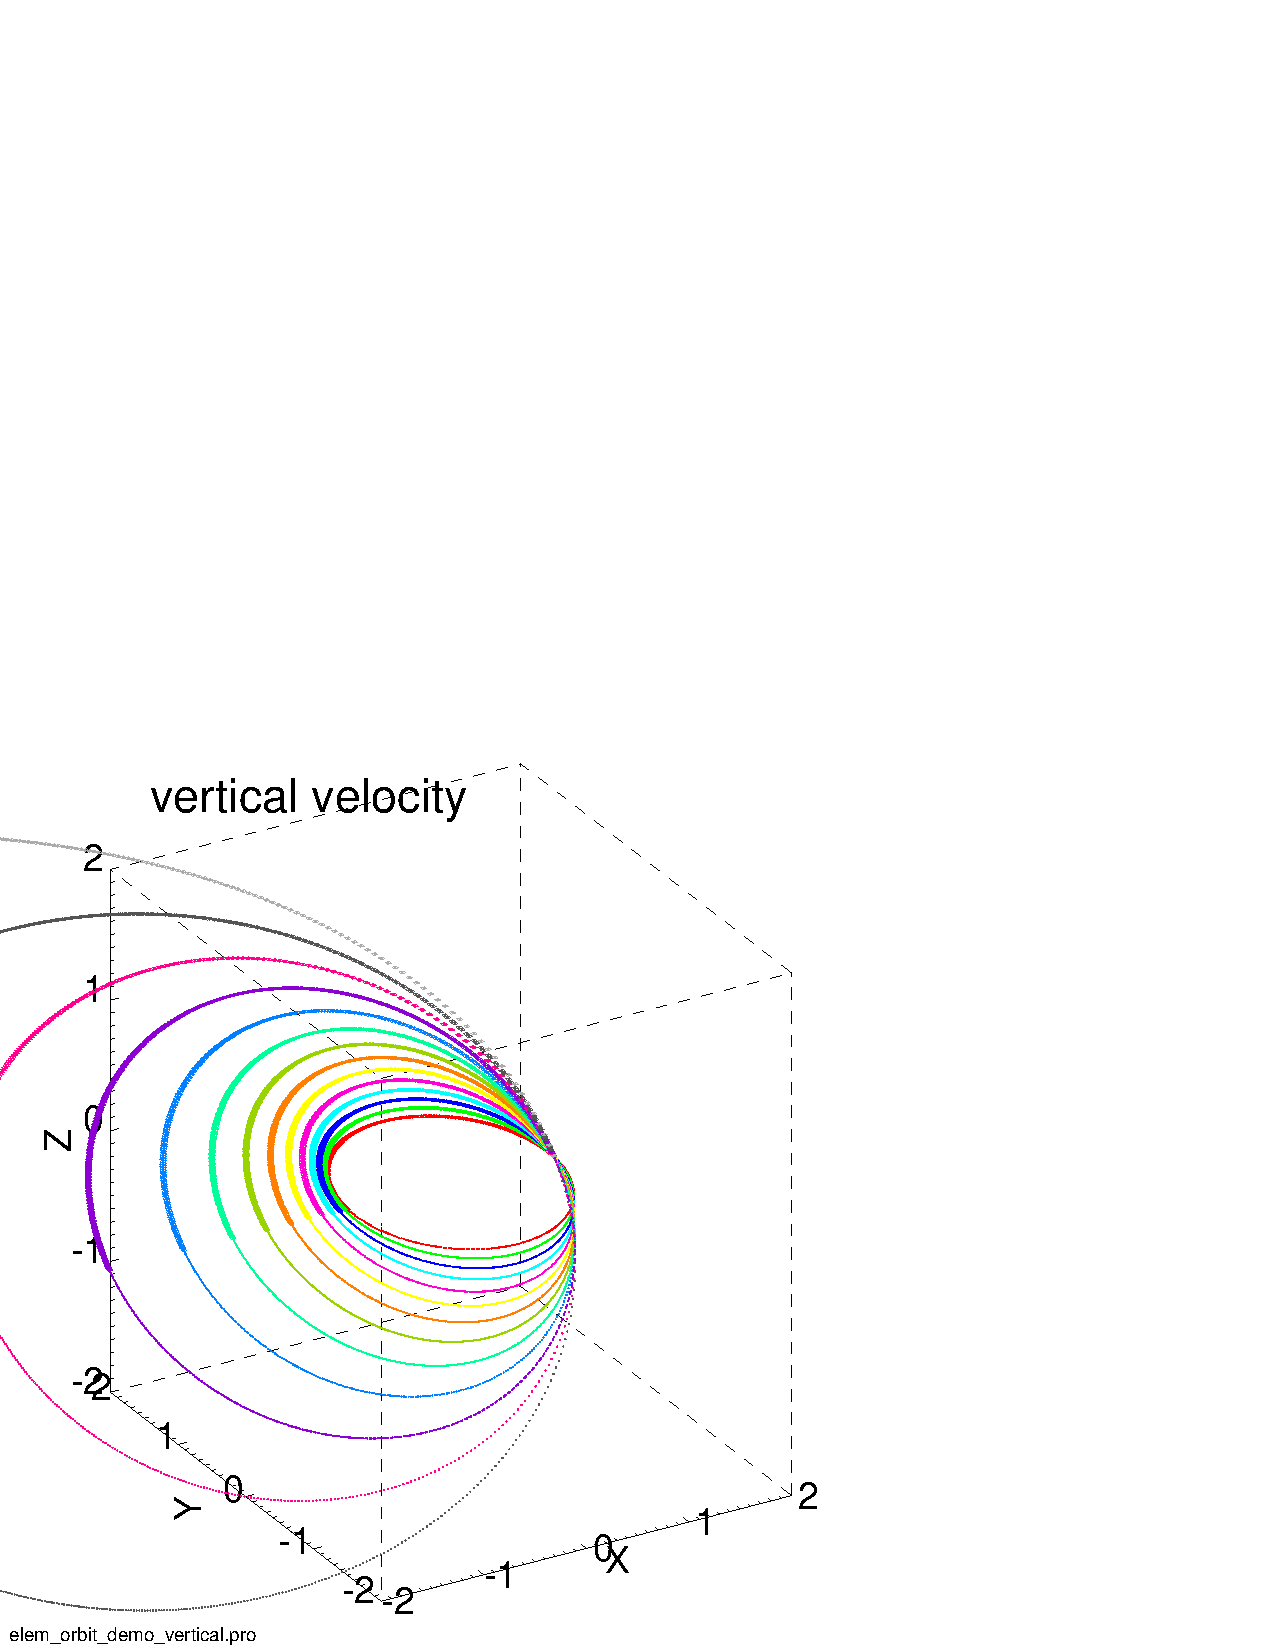
\includegraphics[height=0.8\paperwidth]{demo_apu2.pdf}

\newpage
\black
\bul 
Launch satellite at different angles (HARJ II.1) \framebox{\bf elem\_rv\_demo1.pro} 

{\red \scriptsize 
\begin{verbatim}
;************************************
; elem_rv_demo1.pro  = HARJ II.1
; HS 05.11.02/01.11.06
;
;************************************

;**************************************************************
;Earth position (AU) and velocity (km/sec)
;assuming circular orbit with velocity 30 km/sec, f=45 degrees
;**************************************************************
   sinf=sin(45/!radeg)
   cosf=sin(45/!radeg)
   r_earth=[cosf,sinf,0.]
   v_earth=[-sinf,cosf,0.]*30.

;**************************************************************
;units: AU and year -> G(m1+m2)=4*pi^2
;orbital speed of Earth = 30 km/sec   = 2*pi AU/year
;km/sec converted to au/year by multiplying with vscale=(2*pi)/30.
;**************************************************************
   myy=4.*!pi^2
   vscale=(2.*!pi)/30.

;-------------------------------------------------------------
;a) satellite launched from Earth, with velocity dv (km/sec),
;   in perpendicular direction N
;-------------------------------------------------------------
   dv=[0.,0.,15.]
   r=r_earth
   v=v_earth+dv
   v=v*vscale

   print,'-------------------------------------------------'
   print,'PERPENDICULAR INITIAL VELOCITY'
   rv_to_elem,0.,r,v,elem,myy=myy,/print

;-------------------------------------------------------------
;b) satellite launched from Earth, with velocity dv (km/sec),
;   dv perpendicular to radius vector,
;   with angle alpha to N and 90-alpha to V
;-------------------------------------------------------------
   alpha=45.
   sina=sin(45/!radeg)
   cosa=sin(45/!radeg)
   vtan=30.+sina*15.
   vnor=cosa*15.
   v=[-sinf*vtan,cosf*vtan,vnor]
   r=r_earth
   v=v*vscale

   print,'-------------------------------------------------'
   print,'PERPENDICULAR INITIAL VELOCITY, ALPHA=45'
   rv_to_elem,0.,r,v,elem,myy=myy,/print


;-------------------------------------------------------------
;c) satellite launched from Earth, with velocity dv (km/sec),
;   dv perpendicular to radius vector,
;   with angle alpha to N
;-------------------------------------------------------------
   alpha=89.99                  ; in the direction of velocity vector
   sina=sin(alpha/!radeg)
   cosa=cos(alpha/!radeg)
   vtan=30.+sina*15.
   vnor=cosa*15.   
   v=[-sinf*vtan,cosf*vtan,vnor]
   r=r_earth
   v=v*vscale

   print,'-------------------------------------------------'
   print,'INITIAL VELOCITY in the direction of Earth velocity'
   print,'R [AU]     =',r
   print,'V [AU/year]=',v
   rv_to_elem,0.,r,v,elem,myy=myy,/print


;**********************************************************
;d) Calculate the same with different directions of the
;initial velocity alpha=0,1,...,90 degrees
;dv is the absolute value of velocity increment
;**********************************************************
   dv=15.

;plot a,eks,ink, ene, amom as a function of alpha
;make arrays for alpha, a,eks,ink
;rv_to_elem returns: elem=[a,eks,ink,ome,w,tau]

   alpha_tab=findgen(91)*1.
   a_tab=alpha_tab*0.
   e_tab=alpha_tab*0.
   i_tab=alpha_tab*0.

   for i=0,n_elements(alpha_tab)-1 do begin
       alpha=alpha_tab(i)
       sina=sin(alpha/!radeg)
       cosa=cos(alpha/!radeg)
       vtan=30.+sina*dv
       vnor=cosa*dv
       v=[-sinf*vtan,cosf*vtan,vnor]
       r=r_earth
       v=v*vscale
;orbital elements
       rv_to_elem,0.,r,v,elem,myy=myy
       a_tab(i)=elem(0)
       e_tab(i)=elem(1)
       i_tab(i)=elem(2)
   endfor
   
;calculate also angular momentum and energy, 
;take into account the sign for elliptic and hyperbolic
   k_tab=a_tab*abs(1.-e_tab^2)   
   h_tab=-myy/(2*a_tab)
   index=where(e_tab gt 1,count)
   if(count ge 1) then h_tab(index)=-h_tab(index)
   

   !p.multi=[0,3,2]
   nwin   
   plot,alpha_tab,a_tab,xtitle='alpha',ytitle='a'
   plot,alpha_tab,e_tab,xtitle='alpha',ytitle='EKS'
   plot,alpha_tab,i_tab,xtitle='alpha',ytitle='INK'
   plot,alpha_tab,h_tab,xtitle='alpha',ytitle='energy'
   oplot,alpha_tab(index(0))*[1,1],[-30,30],lines=2
   plot,alpha_tab,k_tab,xtitle='alpha',ytitle='angular momentum'
   

   xyouts,0.67,0.40,/normal, 'Particle launched from Earth (v=30 km/s)',chars=0.7
   xyouts,0.67,0.35,/normal,'fixed initial speed='+string(dv,'(f6.2)')+'km/s',chars=0.7
   xyouts,0.67,0.30,/normal, 'velocity perpendicular to radius-vector',chars=0.7
   xyouts,0.67,0.25,/normal, 'alpha= angle from normal direction',chars=0.7
   xyouts,0.67,0.20,/normal, '(alpha=90 -> tangential increment)',chars=0.7
   
xyouts,0.01,0.01,'elem_rv_demo1.pro',/normal,chars=.5
!p.charsize=1
charsize,1
!p.multi=0
end

\end{verbatim}
\black}

\vspace{-14cm}
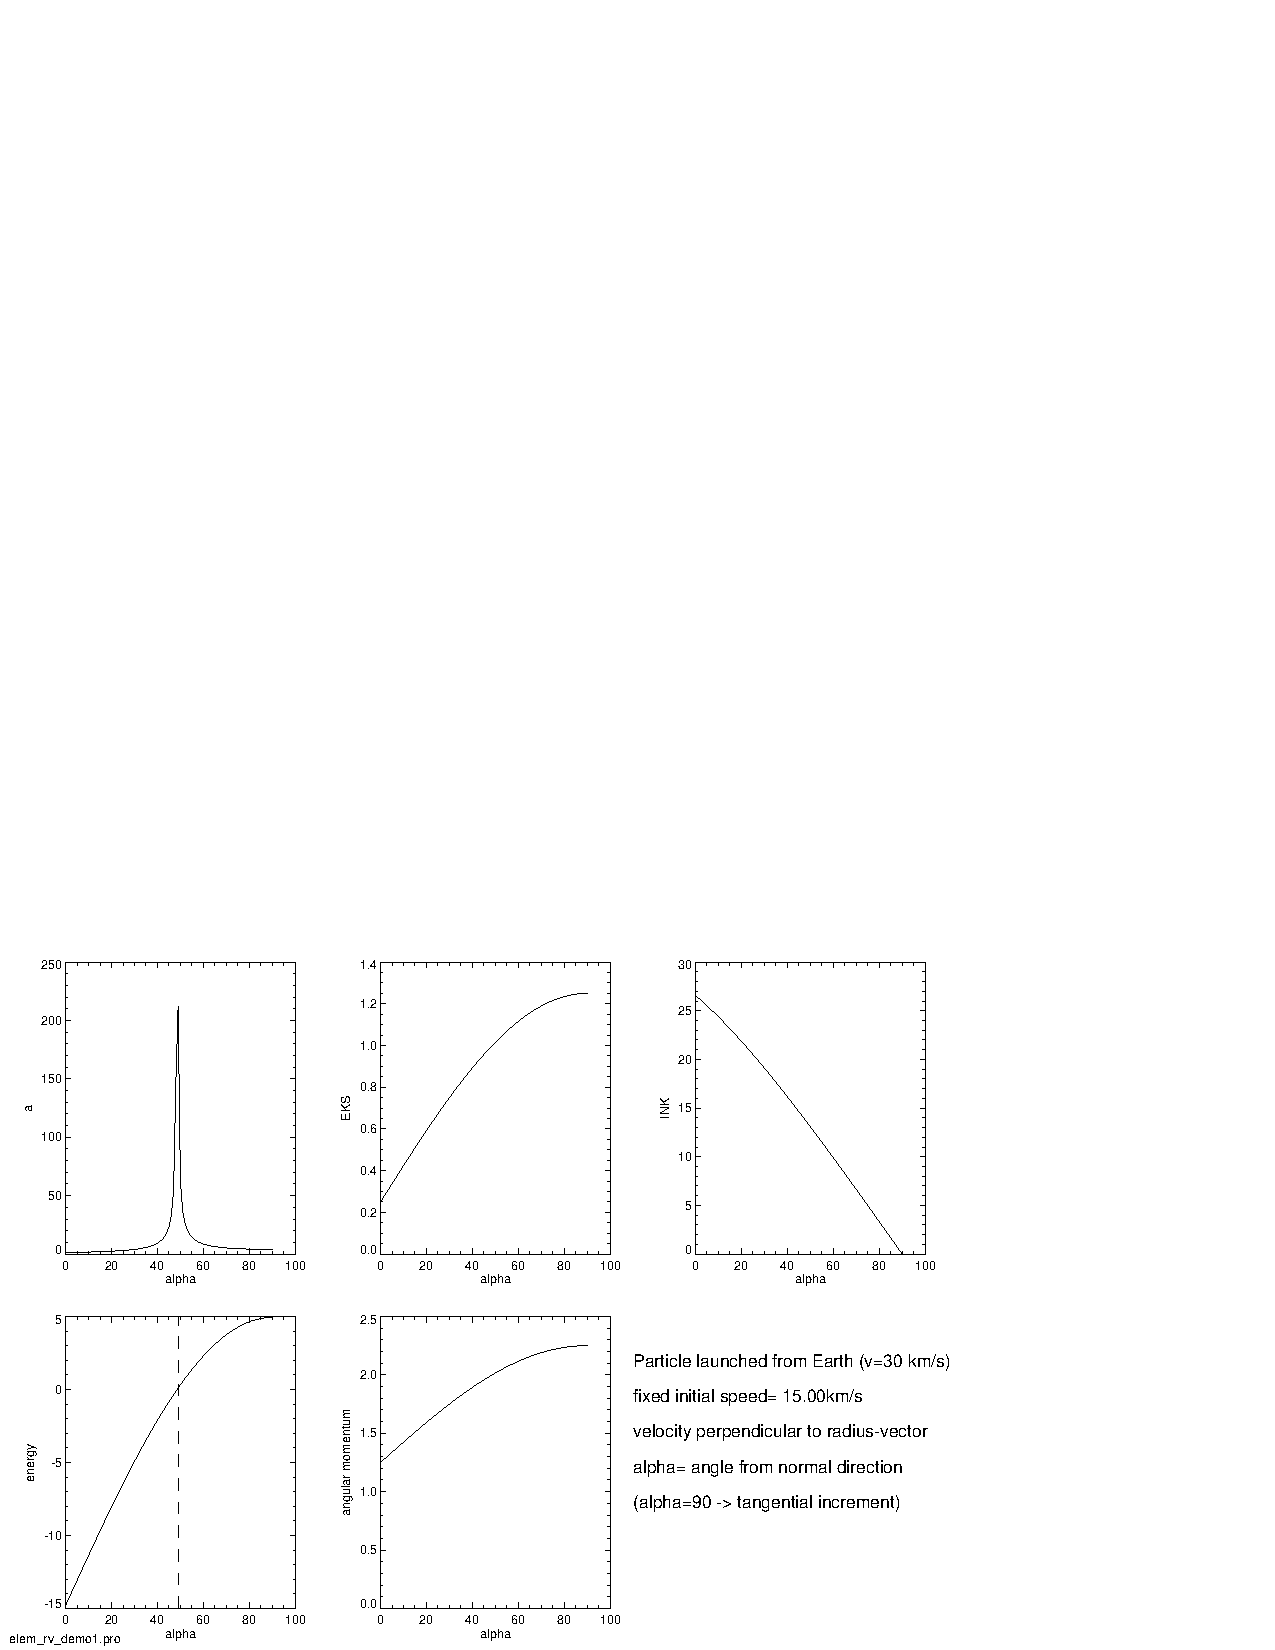
\includegraphics[height=1.23\paperwidth]{elem_rv_demo1.pdf}


\newpage
{\scriptsize
\begin{verbatim}


-------------------------------------------------
PERPENDICULAR INITIAL VELOCITY
-------------------------------------------------
CALCULATED ELEMENTS OF ELLIPTIC ORBIT: at T=      0.00000
a   =        1.3333330
eks =       0.25000000
ink =        26.565052
ome =        45.000000
w   =        0.0000000
tau =   -0.00018333057

per =        1.5396001     0.042867628
q   =       0.99999977

-------------------------------------------------
-------------------------------------------------
PERPENDICULAR INITIAL VELOCITY, ALPHA=45
-------------------------------------------------
CALCULATED ELEMENTS OF ELLIPTIC ORBIT: at T=      0.00000
a   =        23.313564
eks =       0.95710689
ink =        14.638788
ome =        45.000000
w   =        0.0000000
tau =   -0.00067585304

per =        112.56749    0.0021614330
q   =       0.99999131

-------------------------------------------------
-------------------------------------------------
INITIAL VELOCITY in the direction of Earth velocity
R [AU]     =     0.707107     0.707107      0.00000
V [AU/year]=     -6.66432      6.66432  0.000548141
-------------------------------------------------
CALCULATED ELEMENTS OF HYPERBOLIC ORBIT: at T=      0.00000
a   =        4.0000027
eks =        1.2499998
ink =        0.0000000
ome =        45.000000
w   =        0.0000000
tau =   -9.3926329e-05

per =        8.0000078    0.0042266808
q   =       0.99999972

-------------------------------------------------
\end{verbatim}
\black}



\newpage
\black
\bul 
Evolution of a swarm of satellites \framebox{\bf elem\_rv\_demo2.pro} 

{\red \scriptsize 
\begin{verbatim}

;***********************
;elem_rv_demo2.pro
;***********************
;plot the evolution of a swarm of particles launched from Earth

;**************************************************************
;Earth position (AU) and velocity (km/sec)
;assuming circular orbit with velocity 30 km/sec, f=0
;**************************************************************
  r_earth=[1.,0.,0.]
  v_earth= [0.,30.,0.]

;initial launch speed dv, in different directions
;in the plane of Earth's orbit, angle is the direction with 
;respect to x-axis
;try different values!
  dv=5
  pscale=3
;dv=1.
;pscale=2.

;choose the number of particles,
;corresponding launching angles
  npart=3600*.5
  angle_tab=findgen(npart)*360./npart

;**************************************************************
;units: AU and year -> G(m1+m2)=4*pi^2
;orbital speed of Earth = 30 km/sec   = 2*pi AU/year
;km/sec converted to au/year by multiplying with vscale=(2*pi)/30.
;**************************************************************
  myy=4.*!pi^2
  vscale=(2.*!pi)/30.

;*************************************************************
;1) calculate and store orbital elements
;   rv_to_elem returns: elem=[a,eks,ink,ome,w,tau]
;*************************************************************
  elem_tab=fltarr(6,npart)      ; npart different particles
  nwin
  for i=0,n_elements(angle_tab)-1 do begin
      angle=angle_tab(i)
      sina=sin(angle/!radeg)
      cosa=cos(angle/!radeg)
      v=v_earth+[cosa,sina,0]*dv ; rad,tan
      r=r_earth
      v=v*vscale
;orbital elements
      rv_to_elem,0.,r,v,elem,myy=myy
      elem_tab(*,i)=elem
  endfor

;********************************************
;2) start calculating positions
;   plot for different times
;********************************************
;store positions to arrays
  xpos=angle_tab*0.
  ypos=angle_tab*0.
;plotting times
  ntimes=1000
  times=findgen(ntimes)*.05
;  ntimes=9
;  times=findgen(ntimes)*.25+.25

  for j=0,ntimes-1 do begin
      time=times(j)
;earth position (circular orbit)
      x_earth=cos(2.*!pi*time)
      y_earth=sin(2.*!pi*time)      
      for i=0,n_elements(angle_tab)-1 do begin
          elem=elem_tab(*,i)
          elem_to_rv,elem,time,rad,vel,myy=myy
          xpos(i)=rad(0)
          ypos(i)=rad(1)
      endfor      
      plot,xpos,ypos,psym=3,xr=[-1,1]*pscale,yr=[-1,1]*pscale,xs=1,ys=1,/iso,$
        title='dv='+string(dv,'(f6.2)')+'km/sec  T/PER ='+string(time,'(f8.3)')
      plots,x_earth,y_earth,psym=1,symsize=1
      plots,0,0,psym=2,symsize=1 
;if you want to stop between plots - uncomment the next lines
;  answ=''
;  read,answ      
  endfor                        ;end loop over times  
end

\end{verbatim}
\black}


\vspace{-9cm}
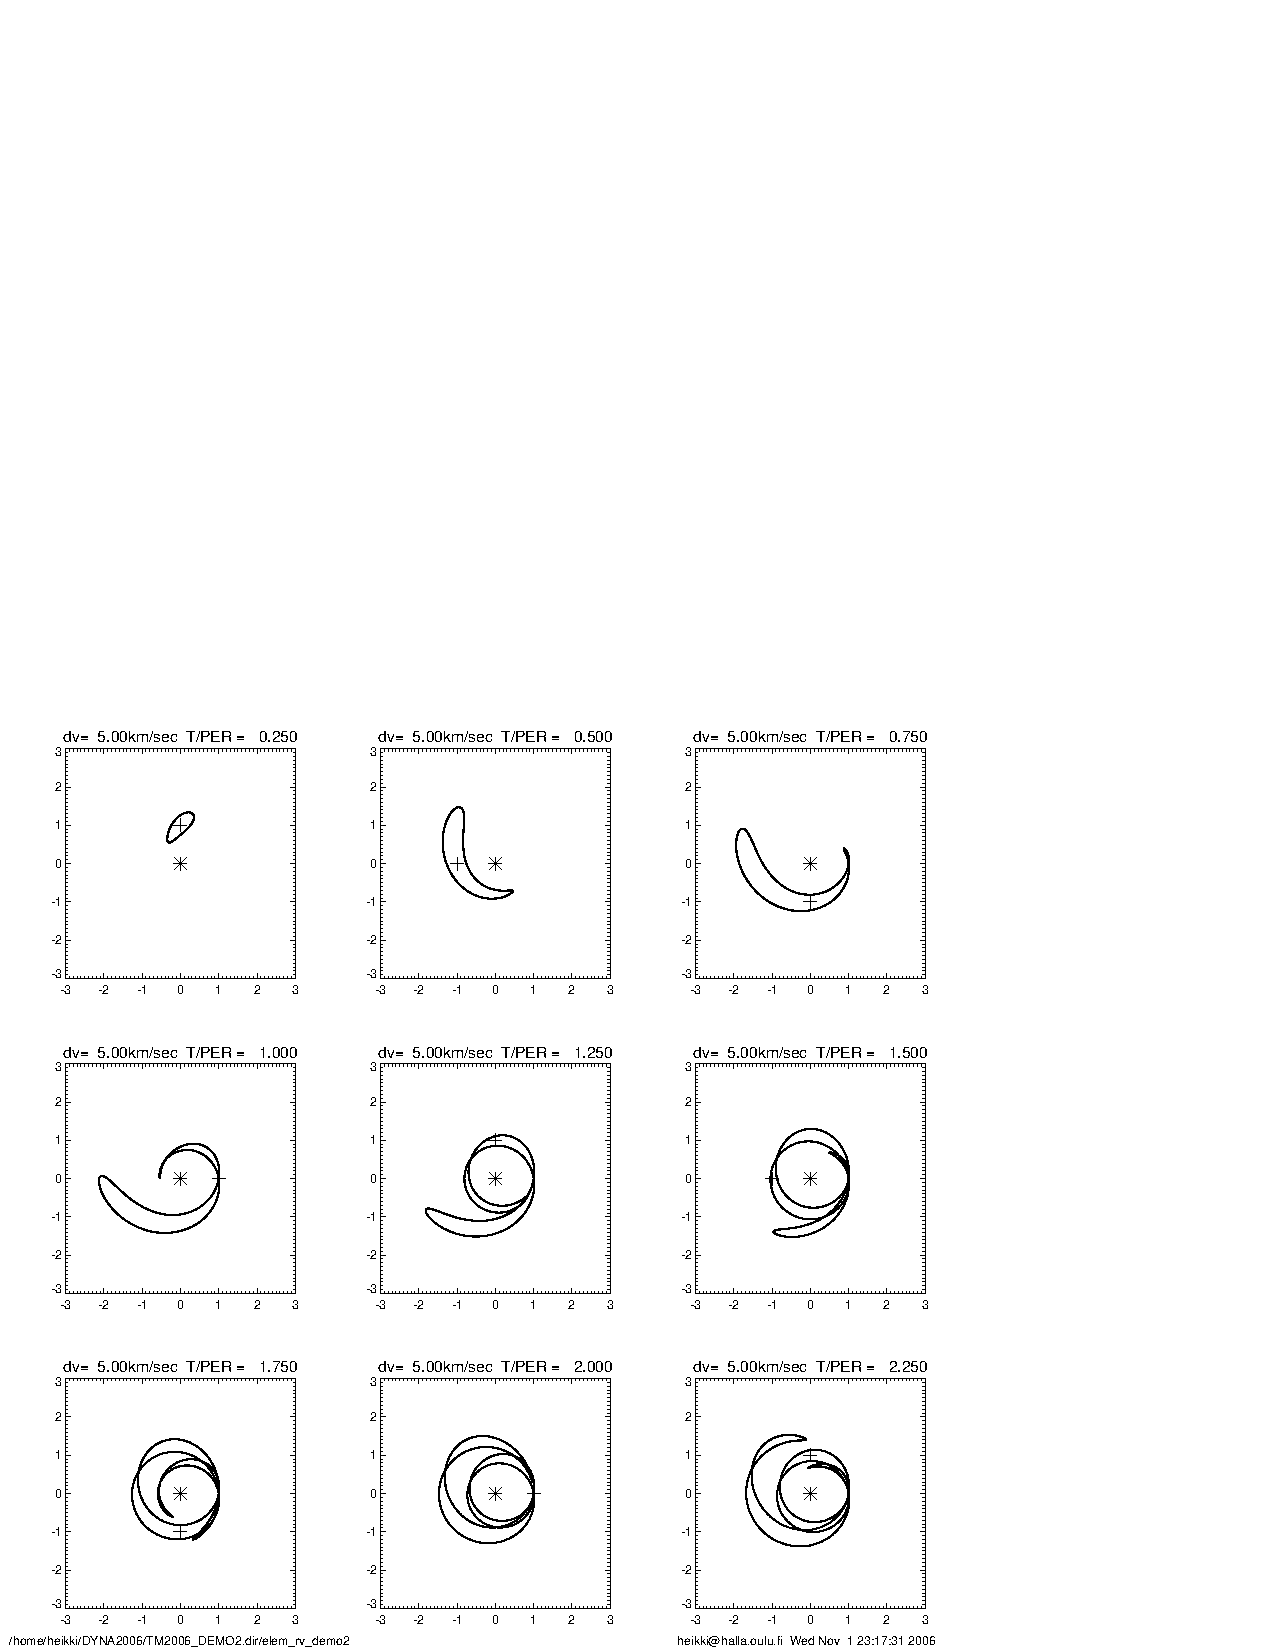
\includegraphics[height=1.\paperwidth]{elem_rv_demo2.pdf}

\end{document}









